\section{Case Study: Shopping Carts}
Applications with replicated state are often concerned with {\em eventual
consistency}.  
%%Broadly, a system with replicated state is eventually consistent
%%if the following conditions are met:
%%\item I
%%Given a system with replicated state, 
%%A system with replicates state is called eventually consistent if we can assert that
Eventually consistent systems are those distributed programs with replicated state for which,
if at some time the system quiesces and all 
messages are delivered, all replicas will have the same state.
In practice, this loose consistency model is desirable because it allows for \emph{asynchronous}
state replication: servers and clients do not
need to wait, or coordinate, to eventually converge to the same state.

%%nrc{I don't see that this is a requirement for EC at all. EC is just a loose consistency model; an 
%%implementation that is consistent with that model may or may not involve asynchrony. E.g., a 
%%strongly consistent system is trivially also ``eventually consistent.''} \wrm{fair enough, 
%%although Joe sez that coordination ``violates the spirit'' of eventual consistency.  so we need 
%%to find some way to work this point in.}
%It follows from this requirement that such systems are ``coordination-free,''
%as in general coordination entails synchrony.
%
%\end{enumerate}

It is not hard to see that eventually consistent programs are a subset of
confluent programs.  First, if coordination is disallowed, 
%%then the program
a program with asynchronously replicated state is either monotonic (commutative, and hence
insensitive to message ordering)
or incorrect.  Second, such a program must be
associative, because two replicas, of which one received a pair of messages in
a single timestamp and the other did not, must achieve the same answer.

In this section, we build a shopping cart application with replicated state,
and reason about the degree to which it is ``eventually consistent.''  Our first 
shopping cart is implemented in a set-oriented style: in the first phase of computation,
changes to the cart are monotonically accumulated and replicated, while in the second
(checkout), the monotonic store is summarized and sealed.  The second shopping cart
is implemented in an imperative, overwriting stytle: as updates are received, the current copy 
is replaced with the new copy.  We then analyze both implementations to identify montonic 
components and state which can be replicated without waiting, and to identify possible
loci of coordination.




\subsection{ACID 2.0}


Helland and others have advocated the design strategy of ensuring eventually-consistent 
semantics for replicated state by enforcing high-level algebraic 
properties in the application logic (in particular, commutativity, associativity and 
idempotence) rather than attempting to provide a RW storage substrate that can provide
such guarantees in general~\cite{quicksand, beyond}.  For example, Dynamo~\cite{dynamo} 
is a RW storage system
and as such needs to provide versioning and conflict resolution capabilities, the shopping
cart application that sits atop it is able to easily reconcile conflicts that occur due to inconsistency of global state, because the application logic is fundamentally order-insensitive.
The eventual state of the shopping cart is guaranteed to be the union of all the operations on
the cart.  In the case of Dynamo, the application logic and not the storage system controls
cart merging logic.

%%Following this reasoning, if our implementation in \lang could be altered in such a way that
%%{\em cart\_update} tuples commute with one another,  we could dispense with the total
%%ordering of tuples.  
Instead of replacing an opaque object as a read/write system would,
we would like to expose the (fundamentally commutative) operation of cart-union to the distributed system.  
%%If this logic were expressed as a user-defined function in the style of SQL databases,
%%we could replace {\em r1} and {\em r2} above with:
%%\begin{Dedalus}
%%persist[cart_update, 3];
%%status(Location, Session, cartunion<CartObj>) \(\leftarrow\)
%%    cart_update(Location, Session, CartObj);
%%\end{Dedalus}
%%But it is only slightly more complicated to hoist the application logic into
%%the server code explicitly.  
To a first approximation, an update to a shopping cart
can be represented as a tuple containing a server and client address, a session identifier,
an item identifier corresponding to goods, a type field that indicates whether this action
is an addition or a deletion, and a request identifier to allow idempotent retry.  The contents
of a shopping cart at checkout time are, for each item referenced in the cart update history, 
the difference between the number of additions and deletions of that item.

\begin{Dedalus}
persist[cart_action, 6];
action_cnt(Location, Session, Item, Type, count<ReqId>) \(\leftarrow\)
    cart_action(Location, Client, Session, Item, Type, ReqId),
    checkout(Location, Client, Session);

status(L, Session, Item, Cnt) \(\leftarrow\)
    action_cnt(L, Session, Item, "Add", Cnt),
    notin action_cnt(L, Session, Item, "Del", _);

status(L, Session, Item, Acnt - Dcnt) \(\leftarrow\)
    action_cnt(L, Session, Item, "Add", Acnt),
    action_cnt(L, Session, Item, "Del", Dcnt);
\end{Dedalus}

The client code generates {\em cart\_action} and {\em checkout} messages in response
to local events.  A sequence is used to uniquely identify {\em cart\_action} requests.

\begin{Dedalus}
// client code
sequence[s, cart_action_stage, 6];
cart_action_stage(Server, Client, Session, Item, Type, ReqId) :-
  action(Client, Session, Item, Type, ReqId),
  best_replica(Client, Session, Server),
  s(ReqId);

cart_action(L, C, S, I, T, R)@async :-
  cart_action_stage(L, C, S, I, T, R);

checkout(Server, Client, Session)@async :-
  checkout_req(Client, Session),
  best_replica(Client, Session, Server);

\end{Dedalus}



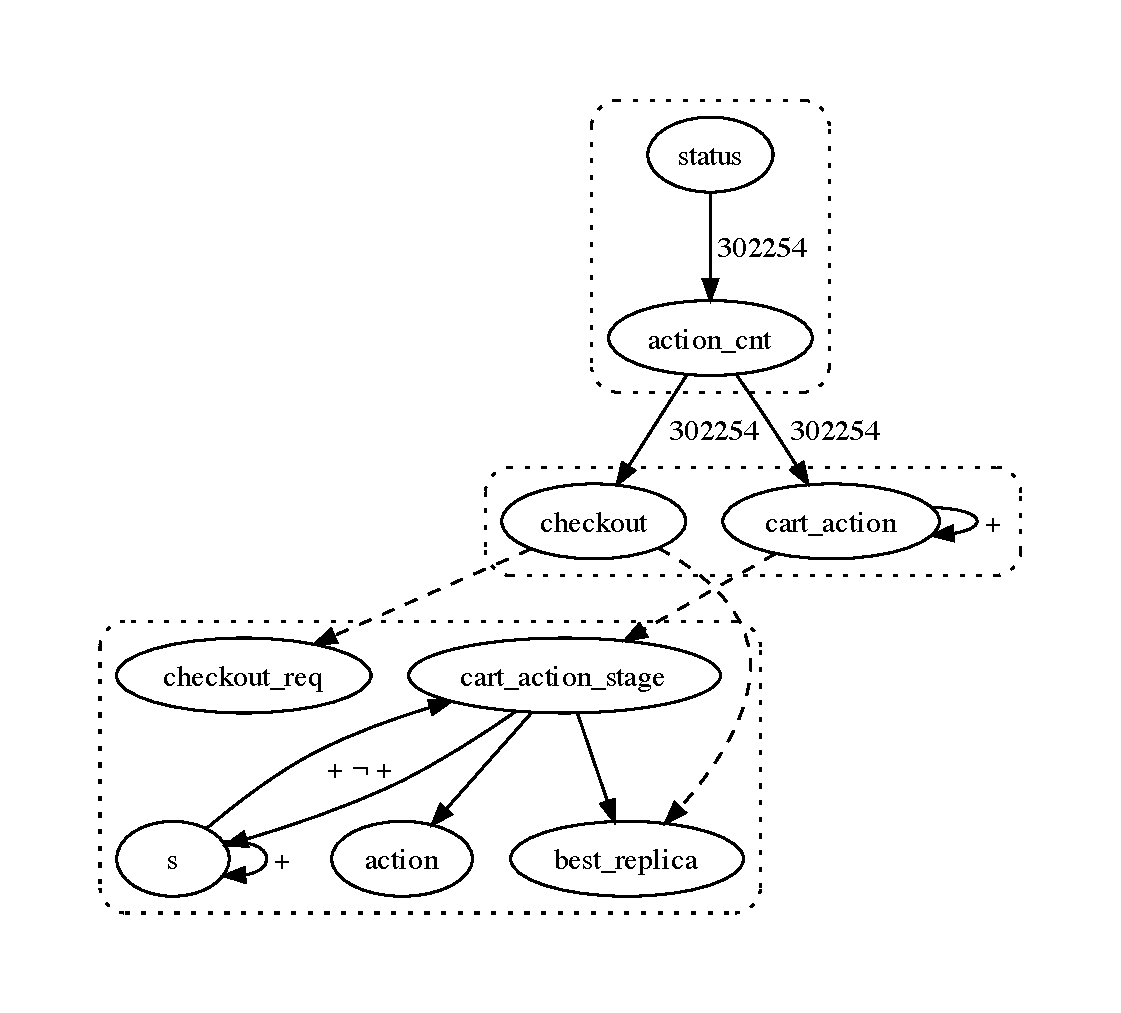
\includegraphics[width=0.9\linewidth]{vizza_brick.pdf}

%%\paa{note that when the graph generation is bug-free, cart\_action should be in the same
%%stratum as cart\_action\_stage -- that is, the stratum crosses a network boundary b/c the
%%async-derived relation cart\_action is naively persisted.  note also that something is
%%jacked up about unicode encoding of $\lnot$.}

%%\wrm{change to PDF when peter commits the shopping cart code to hg}

Our tests immediately show us that the program is not necessarily confluent: 
{\em action\_cnt} falls at a non-local stratification boundary, so it and all tables that
depend on it may be affected by the arrival order of tuples to {\em cart\_action} and
{\em checkout}.  This is not surprising: even though both relations are persisted monotonically,
the arrival of a {\em checkout} tuple may cause us to universally quantify over {\em cart\_action}
at some time $N$, only to have a latecomer {\em cart\_action} tuple arrive at some $M > N$.
There are several options available to the programmer depending on the business rules.
If it is acceptable to ignore the latecomers, the program must merely ensure that they do not 
cause the recalculation of {\em action\_cnt} and transmission of conflicting {\em response} 
tuples.  We can achieve this by using the ``at most once'' pattern, which ``seals'' the value
of $Cnt$ in {\em log} at the first insertion, and ensures that {\em log\_event} occurs once.
\paa{note: introduce the commitfirst macro in the committed choice section of constructs}
\begin{Dedalus}
commitfirst[log, 4, 3];
log(L, Session, Item, Cnt) \(\leftarrow\) 
    status(L, User, Session, Item, Cnt);

response(#Client, Session, Item, Amt)@async \(\leftarrow\)
    log_event(#Location, Session, Item, Amt),
    checkout(#Location, Client, Session);
\end{Dedalus}


If, on the other hand, ignoring late {\em  cart\_update} tuples is not acceptable,
some data dependency between them and {\em checkout} tuples must be established
to ensure that the deduction of {\em action\_cnt} tuples must {\em wait}.  
The ordered queue pattern introduced in (constructs) is one means of achieving such an 
ordering, as is sending a manifest (e.g., a count of total {\em cart\_action} tuples
sent) in the {\em checkout} message.




In addition to illustrating where in our program coordination may be necessary, our
analysis also illustrates where is is unecessary.
The predicate {\em cart\_action}, representing the stored state 
of the cart program,  is part of a monotonic component that includes {\em cart\_action\_stage}, 
so we can simply and inexpensively replicate it:

\begin{Dedalus}
cart_action(#R, S, I, T, Ri)@async :-
    cart_action(#L, S, I, T, Ri),
    replicas(#L, S, R);
\end{Dedalus}

Because {\em cart\_update} is persisted monotonically, it has set semantics over time: at
{\em some} time, when all tuples are received, the order in which they were received is
abstracted away.  Hence asynchronous replication of {\em cart\_update} is confluent,
up to any nonmonotonic operations on the table.


\subsection{Mutable State}

\begin{comment}
What's missing: draw a bold line every place where you see a (-) (negation or aggregation)
or a half-arrow(unguarded asynchrony).  these are the global stratum boundaries, at which
we must either coordinate or commit to a defeasible conclusion to proceed.
crow's feet indicate persistence-guarded asynchrony.  though crow's feet dependencies
may cross network boundaries, they are intra-stratum.
\end{comment}

%%wooden man (straw instrumented with a queue to handle 'coincidence'):
%%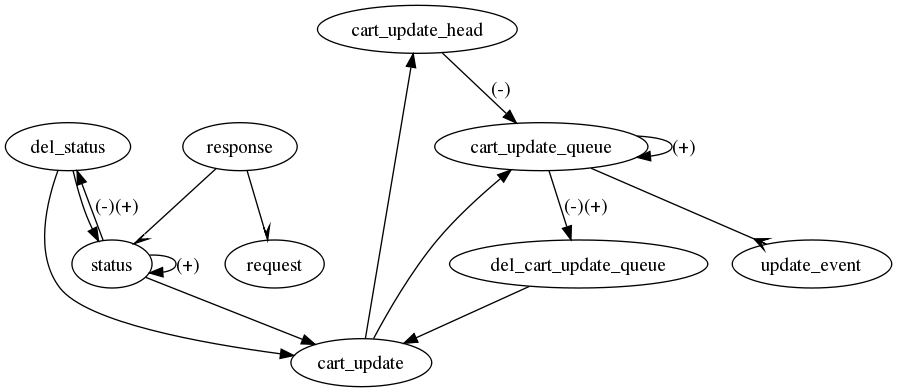
\includegraphics[width=1.2\linewidth]{vizza_wood.png}
%%\wrm{change to PDF when peter commits the shopping cart code to hg}



The simplest imaginable shopping cart implementation behaves like a key-value store,
and treats the cart as an opaque object that is repeatedly updated.    Because we have not
attempted to hoist, as we did in the previous example, application logic about cart merging
into the server code, this implementation is superficially more terse and simple.

\begin{Dedalus}
persist[status, 3];
queue[cart_update, 3, 2];
r1
status(Location, Session, CartObj) \(\leftarrow\)
    cart_update(Location,  Session, CartObj);
    
r2
delete status(L, S, C) \(\leftarrow\)
    status(L, S, C), cart_update(L, S, _);
  
response(#Client, Loc, Session, CartObj) \(\leftarrow\)
    status(#Loc, Session, CartObj),
    request(#Loc, Client, User, Session);

// client code

cart_update(L, S, C)@async \(\leftarrow\) 
    update_event(L, S, C);

\end{Dedalus}

\paa{no longer sure whether the discussion in the below para is worth the space...}
Note that 
{\em cart\_update} is declared using the {\em queue} macro, which expands to
a program fragment that ensures that tuples corresponding to only one $CartObj$
are processed in a single fixpoint. \wrm{note that we desire a primary key...}
Consider the behavior of the program without the queue.  Because {\em
cart\_update} appears in the head of an asynchronous rule,
\dedalus{cart\_update} tuples may be assigned arbitrary timestamps, and some
\dedalus{cart\_update} facts may be assigned the same timestamp, even though
they were derived serially at the sender.  \wrm{this causes some issue because
we have a logic bug in our program...}

%rule in the global program \nrc{What's a ``global program''?}, and hence it is impossible to predict the assignment of timestamps
%to deduced tuples.  Even if the client deduces {\em cart\_update} tuples in a serial manner, it
%is possible for multiple tuples to appear at the receiver in the same timestep \wrm{in other words the bug is that the program isn't correct under associativity of messages}.  Thus rules {\em r1} 
%and {\em r2}, which appear to describe how a single tuple in {\em status} representing a user
%session is updated when a tuple in {\em cart\_update} appears, may cause multiple records
%to appear in {\em status} for the same session (a violation of the implied primary key) \wrm{implied primary key?  we should say earlier ``intuitively we want a primary key'' or something}.
%%To mitigate this bug, we must ensure that exactly one tuple (per session) is available for %%dequeue
%%from {\em cart\_update} at any time.  The \emph{queue} template presented in section ?? 
%%provides this capability.


%replace fancy pants diction -wrm A simple syntactic analysis of the above
%program shows that {\em status} is temporally stratifiable.  but not
%syntactically stratifiable: the deletion rule and the expansion of the
%persistence template define {\em status} in terms of its own negation (in
%time)
%%\wrm{this shouldn't be a surprise to anyone, all the constructs we've presented have this %%property, and we've been harping on this for the previous 2 sections at length}.  


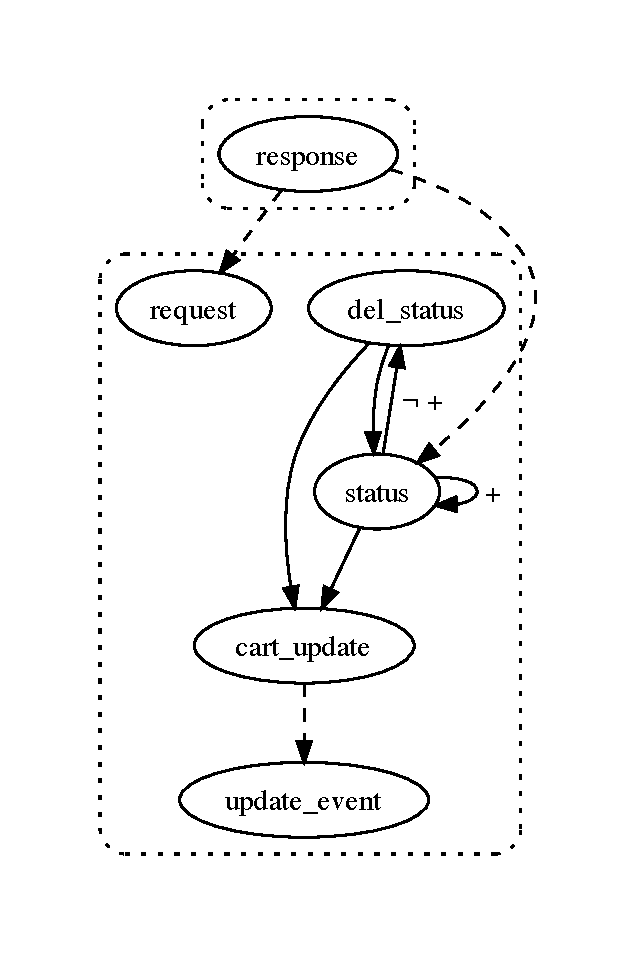
\includegraphics[width=0.65\linewidth]{vizza_straw.pdf}

\paa{another bug: update and cart\_update should be in different strata, b/c
they are separated by an async rule that is NOT ``guarded'' by a persistence rule
associated with its head predicate}

\begin{comment}
what does the analysis tell us?

cart\_update (upon which all other predicates depend) is at a stratum boundary (which 
correponds exactly to a network boundary).  any conclusions drawn from cart\_update
are affected by ND ordering in the channel.  the 'mutability' of cart\_update tuples is
handled via the update pattern (a "TS" instance of nonmonotonicity).  request()s are likewise order-sensitive.  

it is clearly not confluent.  
\end{comment}



Looking at the above program, we can see that {\em status} is defined by the
state update pattern (Section whatever) on {\em cart\_update} -- recall that
the state update pattern means that the ``latest'' tuple ``wins.'' Thus clearly
{\em cart\_update} tuples do not commute with each other
%%, the program is not confluent, 
and the program as
given is unlikely to return the correct version of the cart in a {\em response}
message.  Our PDG analysis confirms this: a stratum boundary separates the client state
(at {\em update} from the server state ({\em cart\_update}), upon which all other 
predicates in the program, including {\em response}, depend.

Considering the {\em cart\_update} tuples in the client's order would solve
this problem.  However, the client's order of the updates is lost through the
asynchronous derivations of {\em cart\_update}, which may arbitrarily reorder
updates.  In Section whatever, we identified the concept of entanglement as a
way to preserve an order in the face of asynchrony.  We can communicate the
desired order from client to server by entangling the sender's time in rule
\dedalus{r4}, and having the server process updates in this order~\footnote{
We could also have used a sequence, if we wanted more control over the range of ordered
values}.
%serial order of updates at the client is lost in the asynchronous derivations
%of {\em cart\_update}.  By entangling the sender's time in rule  {\em r4}, we
%may communicate the desired total order over the {\em cart\_update} tuples and
%process them in that order.
The rest of the code is unchanged, except that an additional argument must be
added to {\em cart\_update}:

\begin{Dedalus}
cart_update_queue(L, S, C, N)@async \(\leftarrow\)
    update_event(L, S, C)@N;
\end{Dedalus}

\wrm{the high level point here is that we've made some bad design choices that
result in us having to over-specify the order.  clearly, a shopping cart doesn't
need this much order because it's commutative, and indeed, we can write it in a
much simpler way.  rusty will insert some points here about how distributing
this naive example results in tons of ugliness (e.g. paxos), and explain that
yes, we could do that in the language if we want (cite netdb).  this will be a
nice contrast with later examples which can be distributed much more easily
because they have much less order and larger monotonic sections.  home run!}
This approach overcomes the nondeterministic ordering implied by asynchronous
communication with brute force: a totally-ordered protocol. This is simple and
inexpensive in this case because it is centralized at the client, obviating the
need for an expensive consensus computation, but the approach has certain
limitations.  First, the client must guarantee that only one {\em
update\_event} is processed per timestep in order to totally order the {\em
cart\_update\_queue} tuples: that is, it must serialize {\em update\_event}
with a queue also.  The matching queues at client and server impose a
synchronization barrier: both sides of the computation must ``spend time''
proportional to the number of tuples.

\rcs{This might be a good place to cite BFS, sherpa, etc.  The para would go something like this (1) if you want to extend the above to multiple writers, then the ordering construct needs to move to the server side.  (2) Once ordering moves to a master node, you need paxos.  (3) in order to replicate you need to allow replicas to send updates to each other.  If you've settled on per-tuple masters, this probably means some sort of log shippinh protocol (a'la our queue, above).  Between the primitives described here and in the bfs/paxos work, you can implement this.  Such systems have been implemented in the past, and are currently in production (CITE PNUTS).  However, such approaches are overkill for shopping carts, and don't show off our nice handling of commutative updates, so:}




\paa{this is too many drawings, but I have to admit I like the drawings and how they illustrate
the componentization of a distributed system into (hopefully maximally large) 'declarative'
components that are order-independent and imperative components}


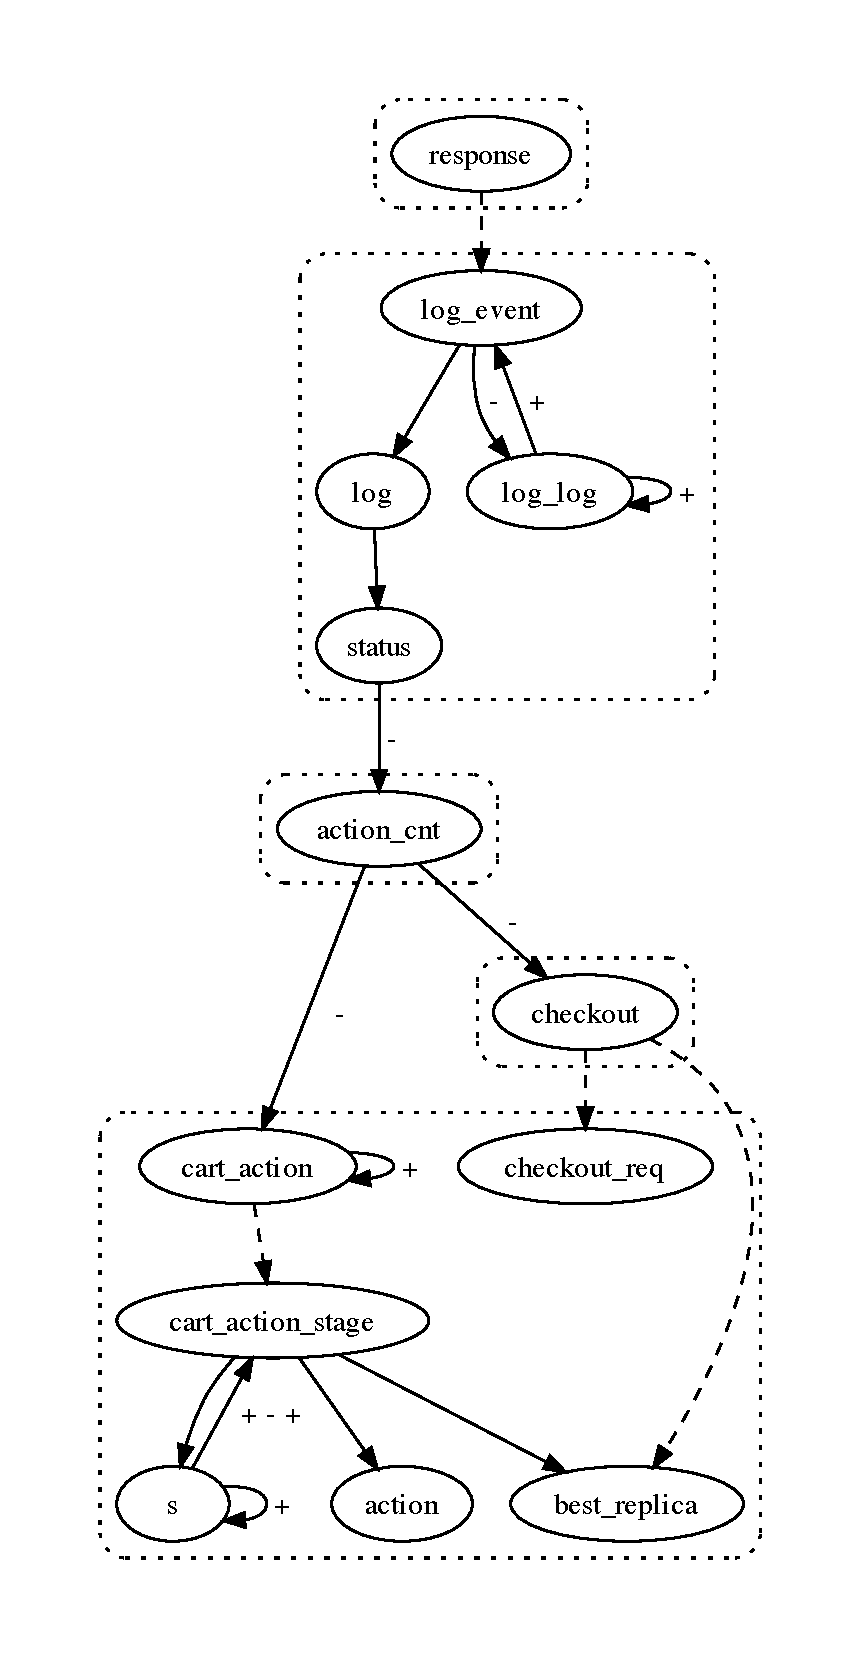
\includegraphics[width=0.65\linewidth]{vizza_withatmostonce.pdf}


\subsection{foo}

... and the client code, just to have it all in here:
\paa{maybe the complete code should just go in an appendix...}

\begin{Dedalus}
commitfirst[publish, 4, 3];

sequence[s, cart_action_stage, 5];
cart_action_stage(#Server, Client, Session, Item, Type, ReqId) \(\leftarrow\)
    action(#Client, Session, Type, ReqId),
    best_replica(#Client, Session, Server);
    s(ReqId);

cart_action(#L, S, I, T, R)@async \(\leftarrow\) 
    cart_action_stage(L, #C, S, I, T, R);

checkout(#Server, Client, Session) \(\leftarrow\)
    checkout_req(#Client, Session),
    best_replica(#Client, Session, Server);
\end{Dedalus}
